

\textbf{Evaluation Plan}

At this point in the thesis, I would have already discussed the results of the combined effect on \textit{single-threaded} performance of different combinations of Vertex-and-edge orderings. The single threaded ``case-study'' will act as a motivation for the next chapters in my thesis (already completed):
    \begin{enumerate}
        \item Parallelization of Slashburn
        \item Parallelization of the edge-centric hilbert traversal via "Hilbert-Blocking"
    \end{enumerate} 

    Since I see this case-study as motivating the main contributions of my research, I don't think I should include it in the evaluation. \newline

    
    % Tentatively, I see the evaluation chapter consisting of 2 main sections.
    % \newline
    % \textbf{Section 1: Ablation Study}
    % An ablation study of the cross-effects and interaction of:
    % \begin{enumerate}
    %     \item vertex ordering
    %     \item edge ordering
    %     \item matrix blocking
    % \end{enumerate}
    % on the performance of \textit{multi-threaded} edge-centric graph traversal (i.e. PageRank computation).
    % This section will answer the following questions:
    % \begin{enumerate}
    %     \item I've shown that there is a performance benefit to be had by combining  vertex-and-edge orderings in the single-threaded setting. How do these speedups translate to the multithreaded setting?
    %     \item For the more time-consuming reorderings, is it even worth it to perform these preprocessing steps?
    % \end{enumerate}
    
    % I'll address (b) by:
    % \begin{enumerate}
    %     \item For each step in the preprocessing pipeline, I would list the preprocessing time and the performance improvement (if any).
    %     \item If I see a speedup, I will also list the number of iterations it would take to amortize the cost of any preprocessing step. 
    % \end{enumerate}
    % It's important to choose a proper baseline here. This could be the ``original'' vertex ID assignment of the input graph (some hyperlink networks that were constructed using crawlers have excellent ``original'' orderings - for these graphs, vertex reorderings have actually been shown to make performance worse).
    % I could also choose a random vertex ordering, or both random and original orderings.

    \par Currently, my plan for the evaluation chapter involves two main sections:

    \textbf{Section 1: Ablation Study}
    
    This section will focus on studying the cross-effects and interaction of vertex ordering, edge ordering, and matrix blocking on the performance of multi-threaded edge-centric graph traversal, specifically PageRank computation. I will answer the following questions:
    
    \begin{itemize}
    \item In the previous sections, I demonstrated that combining vertex-and-edge orderings can improve single-threaded performance. How does this translate to the multithreaded setting?
    \item For more time-consuming reorderings, do the benefits justify the cost of preprocessing?
    \end{itemize}
    
    To address the second question, I will list the preprocessing time and the corresponding performance improvement for each step in the preprocessing pipeline. If there is a speedup, I will also indicate the number of iterations required to amortize the cost of the preprocessing step.
    
    To ensure an appropriate baseline for comparison, I will consider the ``original'' vertex ID assignment of the input graph, which may be the best option for hyperlink networks constructed using crawlers, as vertex reorderings have been shown to decrease performance in some cases. Additionally, I may consider a random vertex ordering, or both random and original orderings.
    
    \textbf{Section 2: Comparison of Runtime, Scaling of Hilbert Blocking and other STOA, in-memory Graph processing systems}

    This section will answer the following:
    \begin{enumerate}
        \item How does Hilbert-Blocking compare to state-of-the-art graph processing systems? 
        \begin{enumerate}
            \item I'll measure runtime and L2, L3 cache miss ratios.
            
        \end{enumerate}
        \item I'll also analyze the scaling behaviours of the different systems.
    \end{enumerate}
    I'll compare against Ligra, Galois, and GPOP.
    It's important to note here that the different systems use different optimizations, whereas my ``optimization'' is more of a preprocessing pipeline: 
    \begin{enumerate}
        \item Vertex Reordering
        \item Edge Reordering and blocking using the Hilbert-Blocks
    \end{enumerate}
    For this reason, I am not sure that it is an apples-to-apples comparison, but still I am able to show some promising results. \newline
    I'll use GPOP as an example for the optimizations these systems use. GPOP partitions the vertices into L2-sized, disjoint vertex sets. It then constructs a graph based on those partitions, with the partitions acting as vertices. If a vertex has multiple neighbours in another partition, GPOP will only send a single update to that partition - this reduces the number of updates written substantially. \newline
    But, as Figure \ref{fig:fig-twitter-comp-illustration} shows, this system doesn't scale well when other vertex orderings have been applied to the graph - specifically ones that make specific regions of the adjacency matrix denser.

    \newpage
    \begin{figure}[!htb]
    \centering
    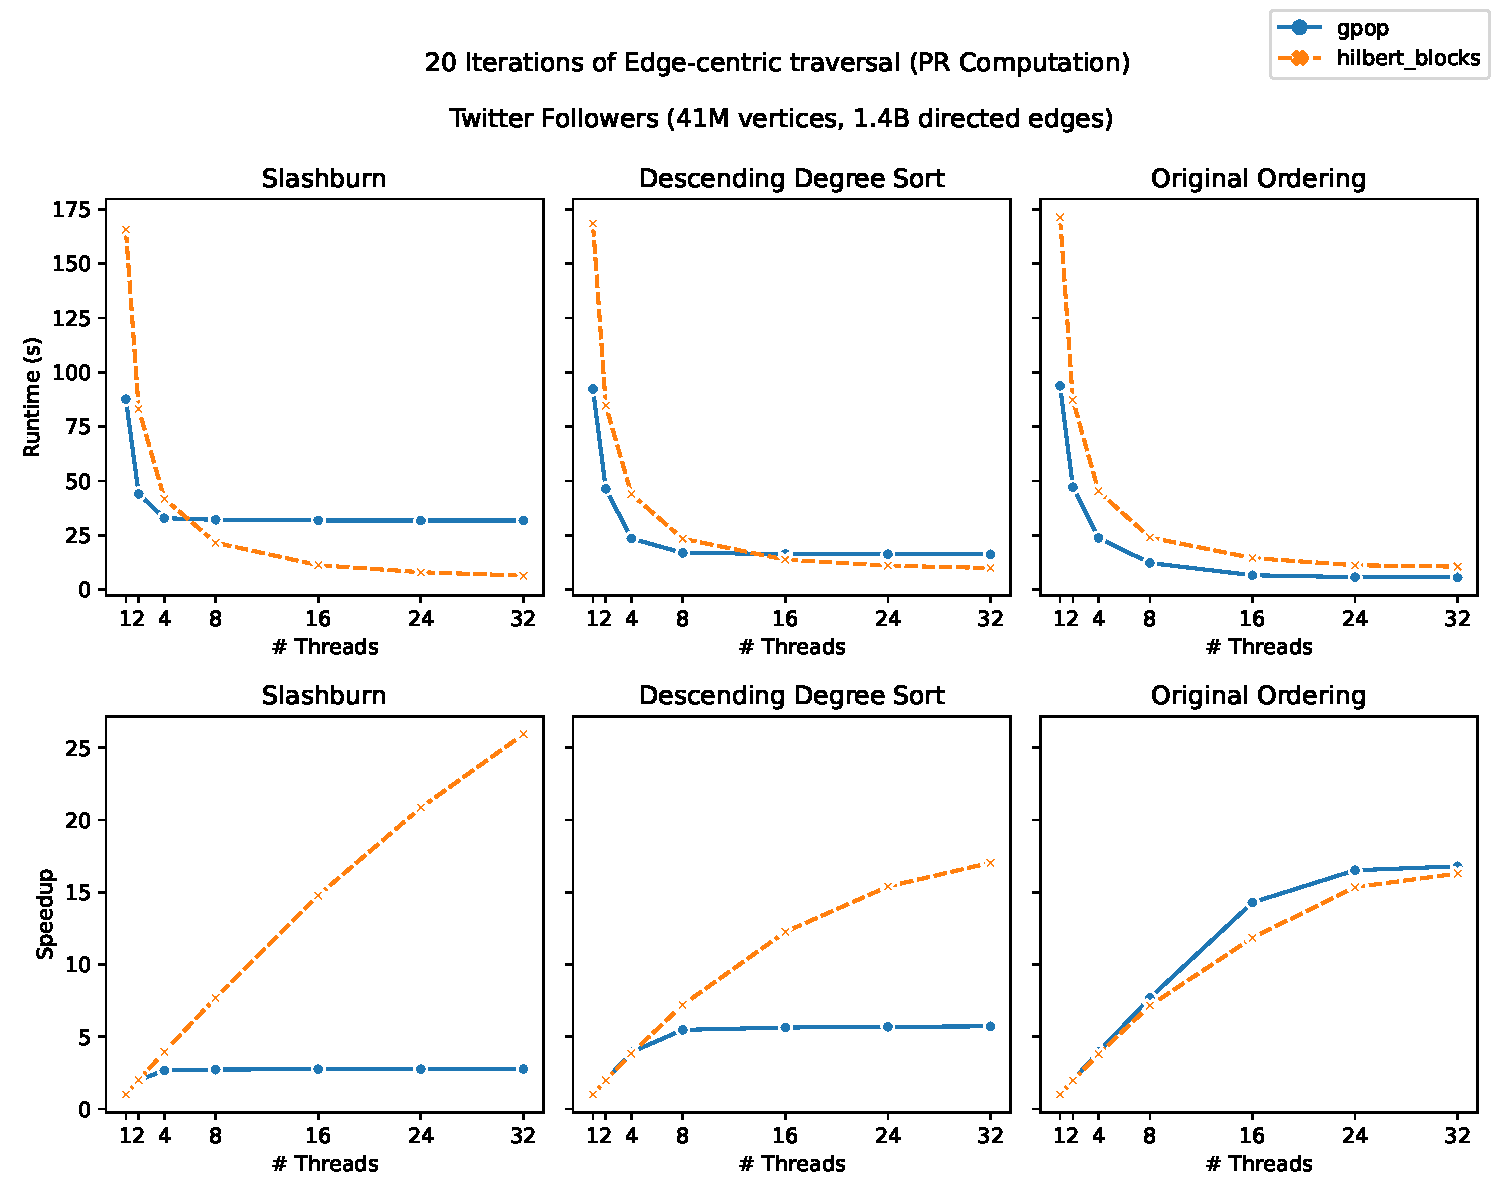
\includegraphics[width=5in]{plots/eval/twitter_gpop_illustrative.pdf}
    \caption{Runtime and Scaling for different vertex reorderings (Original, Descending (Out) Degree Sort, and  Slashburn) for PageRank computation using GPOP and Hilbert Blocking.}
    \label{fig:fig-twitter-comp-illustration}   % label should change
    \end{figure}
    
    \textit{Takeaways from Figure \ref{fig:fig-twitter-comp-illustration}}

    \begin{enumerate}
        \item For vertex reorderings that construct dense areas of the adjacency matrix (Slashburn, Degree sort), 
        GPOP is unable to scale. This is to be expected, since a large proportion of the edges of the graph will be contained within a few partitions - those partitions that contain the high degree vertices of the graph, which are assigned a lower vertex ID value. Since partitions are processed on a per-core basis, the cores that are processing the partitions that contain the high-degree vertices will straggle, while the other cores will be blocked waiting for these cores to finish.
        \item The baseline, single-core performance of Hilbert-blocking is consistently much worse than GPOP.
        Also to be expected, due to the system optimization discussed above. 
        \item The combination of Hilbert blocking and Slashburn produces strong scaling behaviour. I need to experiment further to provide sufficient explanation to why this is. 
        \item The best performing data point is using GPOP on the original twitter graph - $5.581$s. Compared to the best performing data point using Hilbert Blocking and Slashburn - $6.387$s. So, even without any preprocessing steps, GPOP outperforms the best Hilbert-Blocking time (which is especially telling since the Parallel Slashburn computation is lengthy - $\approx$ 20 minutes).
        \begin{itemize}
            \item I'm finding it difficult to construct a meaningful narrative based on these findings, but I think the following may make sense: I mention that vertex reorderings like Descending Degree Sort have been shown to be useful for other workloads (e.g. Triangle Counting). So, 
            if we make the assumption that users would like to store their graph using such a vertex reordering, then these results advocate for the Hilbert Blocking technique.
        \end{itemize}
    \end{enumerate}